\documentclass[11pt]{article}

\usepackage[portuguese]{babel}
\usepackage[utf8]{inputenc}
\usepackage{amsmath}
\usepackage{graphicx}
\usepackage{float}
\usepackage{subfig}
\usepackage{fixltx2e}
\usepackage[bottom]{footmisc}
\usepackage{color}
\usepackage{xargs}                      % Use more than one optional parameter in a new commands
\usepackage[pdftex,dvipsnames]{xcolor}  % Coloured text etc.
\usepackage[colorinlistoftodos,prependcaption,textsize=tiny]{todonotes}
\usepackage{listings}
\usepackage[font=footnotesize]{caption}

\definecolor{keywordcolor}{rgb}{0,0.4,0.7}
\definecolor{commentcolor}{rgb}{0.4,0.4,0.4} 	
\definecolor{mygray}{rgb}{0.5,0.5,0.5} 	% line counter color
\definecolor{mymauve}{rgb}{0.90,0.25,0.47}	% string color
\definecolor{codebackground}{rgb}{0.95,0.95,0.95} 

\newcommandx{\unsure}[2][1=]{\todo[linecolor=red,backgroundcolor=red!25,bordercolor=red,#1]{#2}}
\newcommandx{\change}[2][1=]{\todo[linecolor=blue,backgroundcolor=blue!25,bordercolor=blue,#1]{#2}}
\newcommandx{\info}[2][1=]{\todo[linecolor=OliveGreen,backgroundcolor=OliveGreen!25,bordercolor=OliveGreen,#1]{#2}}
\newcommandx{\improvement}[2][1=]{\todo[linecolor=Plum,backgroundcolor=Plum!25,bordercolor=Plum,#1]{#2}}
\newcommandx{\thiswillnotshow}[2][1=]{\todo[disable,#1]{#2}}
\usepackage[font=footnotesize]{caption}

\numberwithin{equation}{section}

\linespread{1.3}
\usepackage{indentfirst}
\usepackage[top=2cm, bottom=2cm, right=2.25cm, left=2.25cm]{geometry}
\addto\captionsportuguese{\renewcommand{\contentsname}{Índice}}
\lstset{ %
	backgroundcolor=\color{codebackground},   % choose the background color; you must add \usepackage{color} or \usepackage{xcolor}
	basicstyle=\ttfamily \footnotesize,        % the size of the fonts that are used for the code
	breakatwhitespace=false,         % sets if automatic breaks should only happen at whitespace
	breaklines=true,                 % sets automatic line breaking
	captionpos=b,                    % sets the caption-position to bottom
	commentstyle=\color{commentcolor},    % comment style
	deletekeywords={...},            % if you want to delete keywords from the given language
	escapeinside={\%*}{*)},          % if you want to add LaTeX within your code
	extendedchars=true,              % lets you use non-ASCII characters; for 8-bits encodings only, does not work with UTF-8
	keepspaces=true,                 % keeps spaces in text, useful for keeping indentation of code (possibly needs columns=flexible)
	keywordstyle=\color{keywordcolor},       % keyword style
	numbers=left,                    % where to put the line-numbers; possible values are (none, left, right)
	numbersep=5pt,                   % how far the line-numbers are from the code
	numberstyle=\tiny\color{mygray}, % the style that is used for the line-numbers
	rulecolor=\color{black},         % if not set, the frame-color may be changed on line-breaks within not-black text (e.g. comments (green here))
	showspaces=false,                % show spaces everywhere adding particular underscores; it overrides 'showstringspaces'
	showstringspaces=false,          % underline spaces within strings only
	showtabs=false,                  % show tabs within strings adding particular underscores
	stepnumber=1,                    % the step between two line-numbers. If it's 1, each line will be numbered
	%stringstyle=\color{mymauve},     % string literal style
	identifierstyle=\color{mymauve},
	tabsize=2                       % sets default tabsize to 2 spaces
}

\setcounter{tocdepth}{1}


\begin{document}

\begin{titlepage}
\begin{center}

\hfill \break
\hfill \break


\includegraphics[width=0.3\textwidth]{./logo}~\\[1cm]

\textsc{\LARGE Instituto Superior Técnico}\\[0.25cm]
\textsc{\Large Mestrado Integrado em Engenharia Electrotécnica e de Computadores}\\[1.8cm]
\textsc{\huge Arquiteturas Avançadas de Computadores}\\[0.25cm]

{\huge \bfseries Paralisação e aceleração de um programa\\[2cm]}

\begin{tabular}{ l l }
Guilherme Branco Teixeira & \hspace{2mm} n.º 70214\\
Maria Margarida Dias dos Reis & \hspace{2mm} n.º 73099 \\
Nuno Miguel Rodrigues Machado & \hspace{2mm} n.º 74236
\end{tabular}

\vfill

{\large Lisboa, 1 de Junho de 2015} 

\end{center}
\end{titlepage}

\pagenumbering{gobble}
\clearpage

\tableofcontents
\pagebreak

\clearpage
\pagenumbering{arabic}

\section{Introdução}
Pretende-se paralisar e acelerar um algoritmo de \textit{smoothing} usando um processador gráfico como ferramenta de computação paralela. Neste relatório esta demonstrado o algoritmo em CPU, as optimizações necessárias e paralisações essenciais de forma a ter os melhores resultados no GPU.
\section{Implementação no CPU }
Inicialmente o algoritmo proposto foi implementado para correr só no CPU. Para isso, foi transcrito para o código C.
O algoritmo divide-se em duas partes fundamentais:


\begin{itemize}
	\vspace{-3mm}
	\item Criação do sinal amostrado;
	\vspace{-1.5mm}
	\item  \textit{Smoothing}  do sinal amostrado;
\end{itemize}
	\subsection{Criação do sinal amostrado}
	O sinal a ser processado é composto pela soma de dois sinais sinusoidais mais um erro com uma amplitude máxima de $0,1$. 
	Todos os calculos são feitos em \texttt{float}, em primeiro lugar é realizado a alocação da memória de todas as variáveis necessárias para o calculo do sinal de entrada. De seguida está representado o código C em detalhe.
\begin{lstlisting}[language=C]
#define N 10000;
	...

	int main() {
	
	float *x, *y, *yest_cpu, *randomArray;
	...
	
	/*Alocacao de memoria*/
	x = (float *)malloc(N*sizeof(float));
	y = (float *)malloc(N*sizeof(float));
	yest_cpu = (float *)malloc(N*sizeof(float));
	randomArray = (float *)malloc(N*sizeof(float));
	...
	exit(0);
	}
\end{lstlisting}

	A implementação do algoritmo do sinal de entrada é composta por um ciclo que itera o numero de amostras do sinal pretendido. Em primeiro lugar é necessário gerar os valores ao sinal que vai ser processado, estes valores são gerados pela seguinte equação
	\vspace{-3mm}
	\begin{equation}
		X ~= ~i/10; 
	\end{equation}
	de seguida é gerado um valor aleatório entre 1 e -1, simulando o ruído resultante da
	amostragem do sinal. Este valor é gerado pela função \texttt{randn()}, o código da função está representado de seguida, é de salientar que o código foi obtido da Internet, onde este simula a função \texttt{randn()} do MatLab :
	\begin{lstlisting}[language=C]
	float randn()
	{
		float x1, x2, w, y1;
		do
		{
			x1 = (float)(2.0 * rand() / RAND_MAX - 1.0);
			x2 = (float)(2.0 * rand() / RAND_MAX - 1.0);
			w = x1 * x1 + x2 * x2;
		} while (w >= 1.0);
	
		w = (float)sqrt((-2.0 * log(w)) / w);
		y1 = x1 * w;
		return y1;
	}
	\end{lstlisting}
	 Depois de obter os valores de \texttt{X} e do valor aleatório pode-se iterar os valores das amostras do sinal a ser processado. O código de seguida representa o ciclo que itera as amostras de \texttt{X}, do valor aleatório, \texttt{randomArray} e o sinal a ser processado, \texttt{Y}.
	 \begin{lstlisting}[language=C]
	 int main(){
		 for (int i = 0; i < N; ++i) {
			 x[i] = (float)i / 10;
			 randomArray[i] = randn();
			 y[i] = function((float)x[i], (float)randomArray[i]);
		 }
	...
	exit(0);
	}
	 \end{lstlisting}
	 
	
	\subsection{\textit{Smoothing}  do sinal  amostrado}
	
	O algoritmo de \textit{Smooth} para o anulamento do ruído resultante da amostragem do sinal é aplicado segundo a expressão seguinte:
	\vspace{-3mm}
	\begin{equation}
		y_{est}~=~\sum_{i = 0}^{N-1}~\frac{\sum_{k = 0}^{N-1}Kb(x_i,x_k)y_k}{\sum_{k = 0}^{N-1}Kb(x_i,x_k)};
	\end{equation}
	\vspace{-3mm}
	\begin{equation}
	K_b(x_i,x_k)~=~e^{-\frac{(x_i - x_k)^2}{2 b^2}};
	\end{equation}
	A implementação do algoritmo em C baseia-se na utilização de um ciclo para o somatório exterior e outro ciclo para o somatório interior, as funções exponencial \texttt{expf} e potencia de base 2, \texttt{powf}, pertence á biblioteca, \texttt{math.h}. O código seguinte demonstra a utilização dos dois ciclos como tambem a das funções para o calculo do \textit{smoothing}:
	\begin{lstlisting}[language=C]
	int main(){
		float sumA, sumB;
		...
		
		for (int i = 0; i < N; ++i) { //percorrer o yest
			sumA = 0;
			for (int j = 0; j < N; ++j) { //percorer o input dataset
				sumA = sumA + ((expf(-powf((x[i] - x[j]), 2) / (2 * powf(SMOOTH, 2)))) * y[j]);
			}
			sumB = 0;
			for (int j = 0; j < N; ++j)	{ //percorer o input dataset
				sumB = sumB + expf(-powf((x[i] - x[j]), 2) / (2 * powf(SMOOTH, 2)));
			}
			yest_cpu[i] = sumA / sumB;
		}
	
		...
		exit(0);
	}
	\end{lstlisting}
	
	
\section{Implementação no GPU}
A implementação em GPU é dividia em 4 partes:
\begin{itemize}
	\vspace{-3mm}
	\item Alocação da memória;
	\vspace{-1.5mm}
	\item  Envio dos dados do CPU para o GPU;
	\vspace{-1.5mm}
	\item  Iniciação do algoritmo em GPU;
	\vspace{-1.5mm}
	\item  Envio dos dados do GPU para o CPU;
\end{itemize}

\subsection{Alocação da memória}
No inicio da implementação da paralisação em CUDA é necessário alocar a memória total a ser enviada do CPU para o GPU. Neste caso também foi alocado a memória total necessária para guardar o resultado do \textit{smoothing}. De seguida apresenta-se o código para alocação da memória do \textit{device} que com tem o GPU:
	\begin{lstlisting}[language=C]
	int main(){
		float *d_x, *d_y, *d_yest;
		...
		cudaMalloc(&d_x, N*sizeof(float)); 
		cudaMalloc(&d_y, N*sizeof(float));
		cudaMalloc(&d_yest, N *sizeof(float));
		...
		exit(0);
	}
	\end{lstlisting}
 
\subsection{Envio dos dados do CPU/GPU ou GPU/CPU}

Com a memória alocada , o passo seguinte é transferir os dados obtidos na secção 2.1, \texttt{X} e \texttt{Y}, para o \textit{device}. É utilizado a função \texttt{cudaMemcpy}, que pertence à biblioteca \texttt{cuda.h}, recebe o ponteiro de destino e o ponteiro onde está a memória a ser transferida, é necessário definir a dimensão de dados a ser transferidos e por fim é necessário definir o sentido da transferência usando as seguintes mascaras, \texttt{cudaMemcpyHostToDevice} sentido do CPU para o GPU e \texttt{cudaMemcpyDeviceToHost} sentido GPU para o CPU. No código seguinte está implementado a função descrita:
	\begin{lstlisting}[language=C]
	int main(){
		float *x, *y, *yest_cpu,*yest_gpu, *randomArray;
		float *d_x, *d_y, *d_yest;
		...
		/*Envio de dados para o device*/
		cudaMemcpy(d_x, x, N*sizeof(float), cudaMemcpyHostToDevice);
		cudaMemcpy(d_y, y, N*sizeof(float), cudaMemcpyHostToDevice);
		...
		/*Envio de dados para o CPU*/
		cudaMemcpy(yest_gpu, d_yest, N*sizeof(float), cudaMemcpyDeviceToHost);
		...
	exit(0);
	}
	\end{lstlisting}
\subsection{Iniciação do algoritmo em GPU}

Depois de enviar todos os dados para o GPU o \textit{kernel} está pronto para ser invocado. O \textit{kernel} representa o código que vai ser executado pela GPU, este é definido pela declaração \texttt{\_\_global\_\_} antes da função C. Ver código seguinte,
	\begin{lstlisting}[language=C]
	__global__ void funtion_smooth(float *x, float *y, float *yest, int n){
	...
	}
	\end{lstlisting}
Com o \textit{kernel} definido este é executado usando a seguinte configuração, 
	\vspace{-3mm}
	\begin{equation}
NomeDaFuncao~ \textless\textless\textless ~NB,NT ~\textgreater\textgreater\textgreater
	\end{equation}

Onde \texttt{NB} é o numero de blocos a ser lançados no GPU e \texttt{NT} o numero de \textit{threads} por bloco.
	
\section{Técnicas de aceleração e optimização}
O código a ser paralisado é referente à segunda secção, \textit{Smoothing}  do sinal amostrado, do capítulo, Implementação no CPU.
Analisou-se a estrutura do algoritmo e verificou-se a possibilidade de optimização e paralisação dos ciclos. 

\subsection{Optimização}
Analisando o algoritmo proposto identificou-se duas situações principais de optimização, número de ciclos e acesso á memória.
Começou-se então por reduzir o número de ciclos do algoritmo, os dois ciclos interiores podem ser reduzidos a um só, com esta alteração verificou-se que se podia reduzir o acesso á memória. Isto é, como as variáveis \texttt{sumA} e \texttt{sumB} calculam-se da mesma forma tirando a diferença de \texttt{sumA}  ser multiplicada por \texttt{y[i]}. Fez-se a seguinte alteração, a parte comum é calculada em primeira instância e o resultado é guardado numa variável auxiliar, \texttt{sum}. Assim para o calculo de \texttt{sumB} é só necessário aceder a cache e obter os valores \texttt{sumB} e \texttt{sum} e para o calculo de \texttt{sumA} acede de igual forma, vai à cache retirar os valores de \texttt{sumA} e \texttt{sum} e um acesso à memória global, \texttt{y[j]}. O código de seguida demonstra a explicação feita anteriormente:
\begin{lstlisting}[language=C]
for (int i = 0; i < N; ++i) {
	for (int j = 0; j < n ;j++){
		sum = (expf(-powf((x[i] - x[j]), 2) / (2 * powf(SMOOTH, 2))));
		sumA = sumA +  sum* y[j];
		sumB = sumB + sum;
		}
	yest[i] = sumA / sumB;
}
\end{lstlisting}

\subsection{Paralisação dos ciclos}
Analisando a optimização do código anterior verificou-se que pode ser paralisado em duas situações:  
\begin{itemize}
	\vspace{-3mm}
	\item Paralisação do ciclo externo;
	\vspace{-1.5mm}
	\item Paralisação do ciclo externo e interno;
\end{itemize}
Para melhor compreensão, no código seguinte está representado qual o ciclo externo e qual o ciclo interno.

\begin{lstlisting}[language=C]
for (int i = 0; i < N; ++i) {/*Ciclo Externo*/
	for (int j = 0; j < n ;j++){/*Ciclo Interno*/
		sum = (expf(-powf((x[i] - x[j]), 2) / (2 * powf(SMOOTH, 2))));
		sumA = sumA +  sum* y[j];
		sumB = sumB + sum;
	}
	yest[i] = sumA / sumB;
}
\end{lstlisting}
 
\subsubsection{Paralisação do ciclo externo}
Analisando o ciclo externo verificou-se que não existe dependências de dados sendo por isso a primeira implementação a ser realizada.
Assim sendo cada iteração do ciclo externo é executada pelas \textit{threads} dos blocos chamados. Como o GPU utilizado é composto por 1024 \textit{threads} por bloco, quando se pretende processar \texttt{N} iterações é necessário saber o número de blocos a serem chamados para isso divide-se o número máximo de iterações pelo número máximo de \textit{threads} por blocos. De seguida está implementado o o código do \textit{kernel} que corre no GPU e a função de chamada pelo CPU.

\begin{lstlisting}[language=C]

__global__ void funtion_smooth(float *x, float *y, float *yest, int n){
	int i = blockIdx.x* blockDim.x + threadIdx.x;
	float sumA=0.0, sumB=0.0,sum=0.0;

	if (i < n){
		for (int j = 0; j < n ;j++){
			sum = (expf(-powf((x[i] - x[j]), 2) / (2 * powf(SMOOTH, 2))));
			sumA = sumA +  sum* y[j];
			sumB = sumB + sum;
		}
		yest[i] = sumA / sumB;
	}
}
int main() {
	...
	dim3 dimBlock(BLOCK_SIZE, 1, 1);
	dim3 dimGrid(N / BLOCK_SIZE + 1, 1, 1);
	funtion_smooth <<< dimGrid, dimBlock >>>(d_x, d_y, d_yest, N);
	...
	exit(0);
}
\end{lstlisting}

O \textit{kernel} a ser executado é composto pelo ciclo interno, ou seja, cada \textit{thread} executa o \textit{smoothing} de cada amostra do sinal. É de salientar que a variável \texttt{i} identifica qual a iteração que o ciclo exterior executava, para isso seguiu-se o seguinte esquema,

\begin{figure}[H]
	\centering
	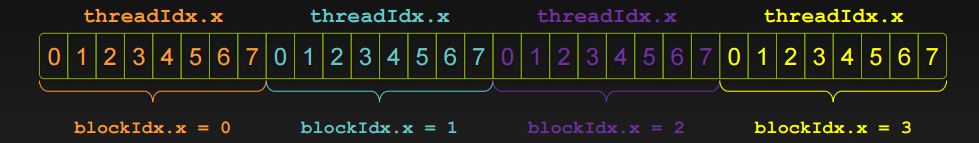
\includegraphics[keepaspectratio=true, scale=0.6]{num_i}
	\vspace{-0.5em}
	\caption{Esquema para indexação única.}
	\vspace{-0.8em}
	\label{fig:imag of i}
\end{figure} 

Como o número de identificação de cada \textit{thread} só identifica a \textit{thread} dentro de cada bloco é necessário obter uma indexação única e igual à do ciclo exterior paralisado. Assim sendo, e analisando a figura anterior obteve-se a seguinte expressão para o calculo do de \texttt{i},  \texttt{i} = \texttt{blockIdx.x}*\texttt{blockDim.x} + \texttt{threadIdx.x};. Onde o \texttt{blockIdx.x} é o identificador do bloco, \texttt{blockDim.x} dimensão de cada bloco e \texttt{threadIdx.x} é o identificador de cada \textit{thread}. 
\subsubsection{Paralisação do ciclo interno}
Ao contrário do ciclo externo o ciclo interno tem dependência de dados dificultando assim a paralisação desse mesmo. Para  a paralisação interna optou-se por dividir o número máximo de iterações em quatro partes, reduzindo assim o tempo de processamento em cada \textit{thread}. O código seguinte representa a implementação referida:
 
 \begin{lstlisting}[language=C]
__global__ void funtion_smooth(float *x, float *y, float *yest, int n){
	int i = blockIdx.x* blockDim.x + threadIdx.x;
	int j = 0;
	float sumA=0.0, sumB=0.0,sumA_Total=0.0, sumB_Total=0.0, sum = 0.0; 
	__shared__ float sumA_partial[BLOCK_SIZE];
	__shared__ float sumB_partial[BLOCK_SIZE];
	
	if ((i/MULTHREADS) < n){
		if(!(threadIdx.x&0x02)){
			if(!(threadIdx.x&0x01)){
				for (j = 0; j < (n/MULTHREADS); j++){
					sum = (expf(-powf((x[i>>2] - x[j]), 2) / (2 * powf(SMOOTH, 2))));
					sumA = sumA + sum* y[j];
					sumB = sumB + sum;
				}
			}else{
				for (j = (n/MULTHREADS); j < 2*(n/MULTHREADS); j++){
					sum = (expf(-powf((x[i>>2] - x[j]), 2) / (2 * powf(SMOOTH, 2))));
					sumA = sumA + sum* y[j];
					sumB = sumB + sum;
				}
			}	
		}else{
			if(!(threadIdx.x&0x01)){
				for (j = 2*(n/MULTHREADS); j < 3*(n/MULTHREADS); j++){
					sum = (expf(-powf((x[i>>2] - x[j]), 2) / (2 * powf(SMOOTH, 2))));
					sumA = sumA + sum* y[j];
					sumB = sumB + sum;
				}
			}else{
				for (j = 3*(n/MULTHREADS); j < 4*(n/MULTHREADS); j++){
					sum = (expf(-powf((x[i>>2] - x[j]), 2) / (2 * powf(SMOOTH, 2))));
					sumA = sumA + sum* y[j];
					sumB = sumB + sum;
				}
		}
	}
	sumA_partial[threadIdx.x]= sumA;
	sumB_partial[threadIdx.x]= sumB;
	...
}
 \end{lstlisting}
 
Como se pode verificar no código anterior, existe quatro ciclos com um quarto do número máximo de iterações. Ao dividir o processamento em quatro \textit{threads} é necessário ter uma memória partilhada:

\begin{lstlisting}[language=C]
__global__ void funtion_smooth(float *x, float *y, float *yest, int n){
...
	__shared__ float sumA_partial[BLOCK_SIZE];
	__shared__ float sumB_partial[BLOCK_SIZE];
...
}
\end{lstlisting}

Para que a organização de cada \textit{thread} seja executa de forma correcta é necessário organizar as \textit{threads} de forma coerente, assim sendo é verificado os últimos dois \textit{bits} menos significativos da variável \texttt{thread.idx} de forma a executar o ciclo correcto, por exemplo, se a variável \texttt{thread.idx} for igual a 1 então executa o 2 ciclo.

Com os dados guardados na memória partilhada é necessário sincronizar todo de forma a obter o resultado acumulado final. Para a sincronização é o utilizado a função de sistema \texttt{\_\_syncthreads();}, que sincroniza todas as \textit{threads} do mesmo bloco.
Depois da sincronização pode-se acumular os resultados de todas as quatro \textit{threads} para isso é utilizado a \textit{thread} que tem os dois \textit{bits} menos significativos a zero, ou seja, a primeira \textit{thread} de cada grupo de quatro. De seguida está demonstrado o código:

\begin{lstlisting}[language=C]
	...
	if(!(threadIdx.x&0x03)){
		for(int l=0 ; l<MULTHREADS;l++){
		sumA_Total += sumA_partial[threadIdx.x + l];
		sumB_Total += sumB_partial[threadIdx.x + l];	
	}
	yest[i>>2] = sumA_Total / sumB_Total;
}
\end{lstlisting}


\section{Secção de resultados}
Depois da implementação anteriormente referida foi analisado os tempos de execução
\subsection{Tempos}
Para o cálculo dos tempos foi usado a função \texttt{clock\_gettime()} e a função \texttt{timeDiff()}. Todas as estruturas e funções não representadas estão na biblioteca \texttt{sys/time.h}.
\begin{lstlisting}[language=C]
	double timeDiff(struct timespec tStart, struct timespec tEnd)
	{
	struct timespec diff;
	
	diff.tv_sec = tEnd.tv_sec - tStart.tv_sec - (tEnd.tv_nsec<tStart.tv_nsec ? 1 : 0);
	diff.tv_nsec = tEnd.tv_nsec - tStart.tv_nsec + (tEnd.tv_nsec<tStart.tv_nsec ? 1000000000 : 0);
	
	return ((double)diff.tv_sec) + ((double)diff.tv_nsec) / 1e9;
	}
\end{lstlisting}
Para o calculo do tempo de execução em CPU foi calculado o intervalo de tempo desde a primeira iteração do ciclo exterior até á ultima tiração.
\begin{lstlisting}[language=C]
int main(){
	...
	struct timespec timeVect[7];
	double timeCPU;
	...
	clock_gettime(CLOCK_REALTIME, &timeVect[0]);/*Inicio da contagem do tempo*/
	
	for (int i = 0; i < N; ++i) { //percorrer o yest
		sumA = 0;
		for (int j = 0; j < N; ++j) { //percorer o input dataset
			sumA = sumA + ((expf(-powf((x[i] - x[j]), 2) / (2 * powf(SMOOTH, 2)))) * y[j]);
		}
		sumB = 0;
		for (int j = 0; j < N; ++j)	{ //percorer o input dataset
			sumB = sumB + expf(-powf((x[i] - x[j]), 2) / (2 * powf(SMOOTH, 2)));
		}
		yest_cpu[i] = sumA / sumB;
	}
	clock_gettime(CLOCK_REALTIME, &timeVect[1]);/*Fim da contagem do tempo*/
	timeCPU = timeDiff(timeVect[0], timeVect[1]);
	printf("    ... execution took %.6f seconds\n", timeCPU);
	...
	exit(0);
}
\end{lstlisting}

O calculo do tempo de execução do GPU referido foi obtido somando o tempo de alocação de memória, o tempo de transferência de dados do CPU para o GPU, o tempo de execução do \textit{kernel} e a transferência dos resultados do GPU para o CPU.
\begin{lstlisting}[language=C]
int main(){
...
	struct timespec timeVect[7];
	double timeCPU,timeGPU[7];
	...
	clock_gettime(CLOCK_REALTIME, &timeVect[1]);/*Inicializacao do contador*/
	
	cudaMalloc(&d_x, N*sizeof(float));
	cudaMalloc(&d_y, N*sizeof(float));
	cudaMalloc(&d_yest, N *sizeof(float));
	clock_gettime(CLOCK_REALTIME, &timeVect[2]);/*Tempo de alocacao de memoria*/
	
	cudaMemcpy(d_x, x, N*sizeof(float), cudaMemcpyHostToDevice);
	cudaMemcpy(d_y, y, N*sizeof(float), cudaMemcpyHostToDevice);
	clock_gettime(CLOCK_REALTIME, &timeVect[3]);/*Tempo de transferencia de dados CPU/GPU*/
	
	dim3 dimBlock(BLOCK_SIZE, 1, 1);
	dim3 dimGrid(N / BLOCK_SIZE + 1, 1, 1);
	
	funtion_smooth <<< dimGrid, dimBlock >>>(d_x, d_y, d_yest, N);
	clock_gettime(CLOCK_REALTIME, &timeVect[4]);/*Tempo de execucao do kernell*/
	
	cudaMemcpy(yest_gpu, d_yest, N*sizeof(float), cudaMemcpyDeviceToHost);
	clock_gettime(CLOCK_REALTIME, &timeVect[5]);/*Tempo de transferencia de dados GPU/CPU*/
	...
	exit(0);
}
\end{lstlisting}
\subsubsection{Paralisação do ciclo externo}
De seguida está implementado uma tabela com os resultados dos tempos de execução da paralisação do ciclo externo em função do número de amostras. Também se encontra representado  na tabela o valor do \textit{speed-up} obtido com a implementação do GPU.
O \textit{speed-up} é calculado pela seguinte equação, $tmp_{cpu}$ tempo de execução no CPU e $tmp_{gpu}$ tempo de execução no GPU.
\vspace{-3mm}
\begin{equation}
	speedup~=~\frac{tmp_{cpu}}{tmp_{gpu}};
\end{equation}

\begin{table}[H]
	\centering
	\caption{Valores dos tempos de execução no CPU e GPU para diferentes valores de amostras.}
	\vspace{-1.5mm}
	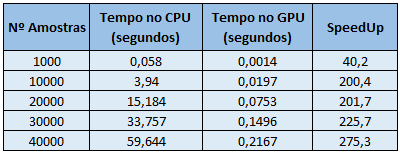
\includegraphics[keepaspectratio=true, scale=0.8]{speedup}
\end{table}

De seguida também está implementado o gráfico do \textit{speed-up} em função do número de amostras.
\begin{figure}[H]
	\centering
	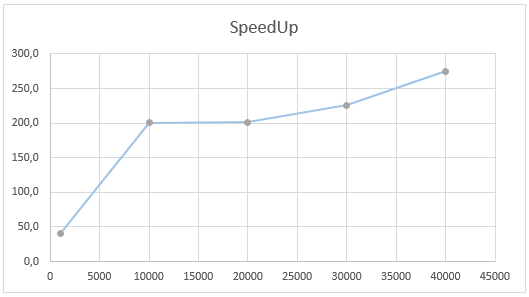
\includegraphics[keepaspectratio=true, scale=0.6]{graficodospeedup}
	\vspace{-0.5em}
	\caption{Gráfico do \textit{speed-up} em função das amostragem.}
	\vspace{-0.8em}
	\label{fig:imag of i}
\end{figure} 

\subsubsection{Paralisação do ciclo externo e interno}
 Está representado os resultados dos tempos de execução referentes á paralisação do ciclo externo e interno. Também se encontra representado  na tabela o valor do \textit{speed-up} obtido com a implementação do GPU.
 O \textit{speed-up} é calculado pela equação anterior 5.1.
 
 \begin{table}[H]
 	\centering
 	\caption{Valores dos tempos de execução no CPU e GPU para diferentes valores de amostras.}
 	\vspace{-1.5mm}
 	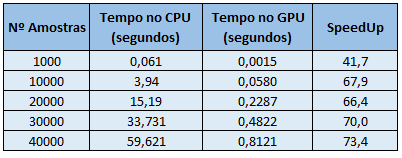
\includegraphics[keepaspectratio=true, scale=0.8]{speedup2}
 \end{table}
 
 De seguida também está implementado o gráfico do \textit{speed-up} em função do número de amostras.
 \begin{figure}[H]
 	\centering
 	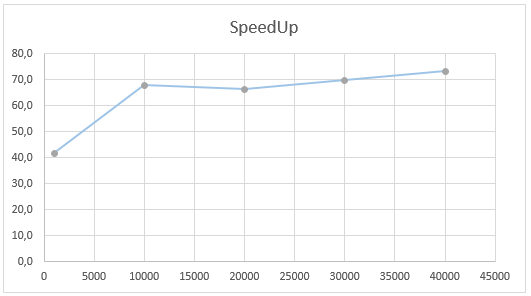
\includegraphics[keepaspectratio=true, scale=0.6]{graficodospeedup2}
 	\vspace{-0.5em}
 	\caption{Gráfico do \textit{speed-up} em função das amostragem.}
 	\vspace{-0.8em}
 	\label{fig:imag of i}
 \end{figure} 
 

\subsection{Resultados do \textit{Smooth}}
Está representado nos gráficos seguintes os resultados das amostras processadas pelo CPU e GPU com 20000 amostras.
\begin{figure}[H]
	\centering
	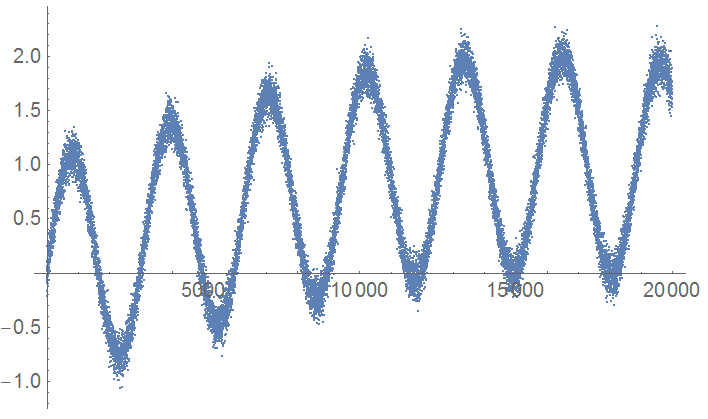
\includegraphics[keepaspectratio=true, scale=0.6]{print2}
	\vspace{-0.5em}
	\caption{Gráfico do sinal amostrado com ruído.}
	\vspace{-0.8em}
	\label{fig:imag of i}
\end{figure} 

\begin{figure}[H]
	\centering
	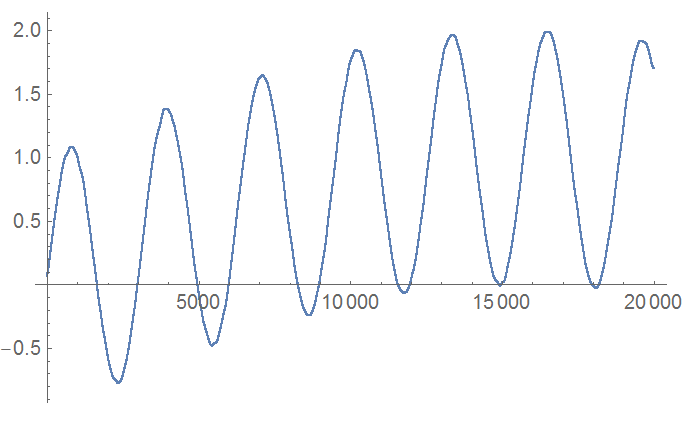
\includegraphics[keepaspectratio=true, scale=0.6]{print1}
	\vspace{-0.5em}
	\caption{Gráfico do sinal amostrado com \textit{smoothing} do ruído implementado em CPU.}
	\vspace{-0.8em}
	\label{fig:imag of i}
\end{figure} 

\begin{figure}[H]
	\centering
	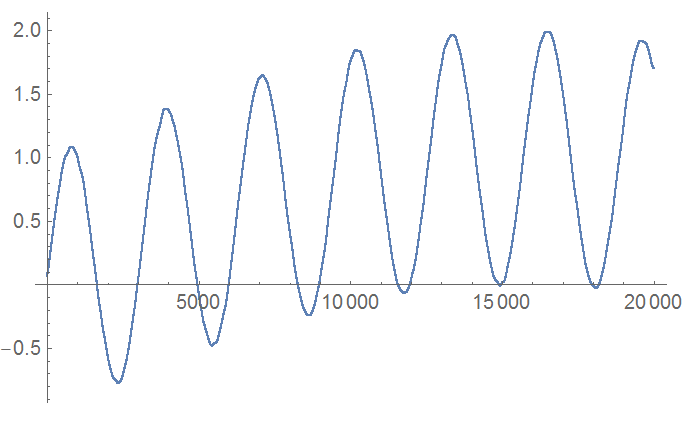
\includegraphics[keepaspectratio=true, scale=0.6]{print1}
	\vspace{-0.5em}
	\caption{Gráfico do sinal amostrado com \textit{smoothing} do ruído implementado em GPU.}
	\vspace{-0.8em}
	\label{fig:imag of i}
\end{figure} 



\section{Conclusões}
 A opitmização escolhida para este algoritmo foi a implementação da paralisação só no ciclo externo, esta escolha é referente aos resultados dos \textit{speed-ups} anteriormente referidos, pois existe um \textit{speed-up} três vezes superior ao da paralisação do ciclo externo e interno. Estes resultado era de esperar devido ao \textit{overhead} que existe na sincronização das\textit{threads} e acesso á memória partilhada. Mesmo com os maus resultados obtidos foi importante implementar esta segunda paralisação devido à complexidade e a utilização de diversas funções do CUDA.
\section{Anexos}
Descrição dos ficheiros em anexo:
\texttt{Smooth\_1v.cu} ficheiro que contem o código da primeira paralisação, paralisação do ciclo externo.
\texttt{Smooth\_2V.cu} ficheiro que contem o código da segunda paralisação, paralisação do ciclo externo e interno.

Na pasta \texttt{Datasets} estão os resultados  obtidos para 1000, 10000 e 20000 amostras.

\end{document}